% ----------------------------- CONCETTI INTERMEDI -----------------------------------

\chapter{Concetti Intermedi}

%Argomenti di questo capitolo: 

% Vari tipi di reinterpret_cast<>, dynamic_cast<>, static_cast<>, const_cast<>
% Lambdas
% Virtual keyword
% Template keyword
% Friend keyword? NO.
% Allocazione dinamica
% Rule of 3 e Rule of 5, Special Member Functions: Copy Constructor, Move Constructor.
% Classi Astratte
% Polimorfismo
% Operazioni su File?
% Exceptions
% RAII
% std::vector<>, dopo questo faccio i templates.

% Operators overload
% Iteratori

% Move semantics

% Map, Set, HashTable, Pair

% #include type_traits

% new e delete

%TODO: decltype.

% Random numbers? O nel beginner?
% std::chrono?

%TODO: inline functions.

%TODO: overloading vs override

%TODO: NULL (o null) vs nullptr

%TODO: perché non usare std::endl ed usare \n piuttosto.

%TODO: steam, std::istream, std::ostream.

%TODO: explicit keyword, converting constructor.

% -------------------------- SECTION: INTRODUZIONE -----------------------------------

\section{Introduzione}

\textsf{\small In questo capitolo, tratterò argomenti non necessariamente più complicati, ma che non considererei basi. } \\

\textsf{\small In questo capitolo vedremo ulteriori concetti riguardo le classi, il polimorfismo, le varie tipologie di costruttori, la programmazione generale, le lambdas, la programmazione funzionale e molto altro ancora..} \break

%TODO: std::vector
%TODO: templates.

% -------------------------- SECTION: TEMPLATES --------------------------------------

\newpage

\section{Templates}

\textsf{\small Immaginiamo di avere un codice, esempio questo:} \\

\begin{lstlisting}
	const int& max(const int& a, const int& b)
	{
		return a > b ? a : b;
	}
\end{lstlisting}

\textsf{\small Però ora se noi volessimo utilizzare questa funzione per i double, dovremmo copiarla e cambiare la tipologia da int a double.} \\

\begin{lstlisting}
	const int& max(const int& a, const int& b)
	{
		return a > b ? a : b;
	}

	const double& max(const double& a, const double& b)
	{
		return a > b ? a : b;
	}
\end{lstlisting}

\textsf{\small C'è un problema, se ora volessimo usare la stessa funzione, ma con i float? o con i char? Certo potremmo fare dei casts, ma così perderemmo dei dati, ma sopratutto ripeteremmo lo stesso codice più e più volte semplicemente per avere la stessa identica funzione, ma per tipologie diverse.} \\

\textsf{\small Inoltre, fare questo, continuare a ripetere lo stesso codice, violerebbe un'importante principio in programmazione, ovvero \textbf{DRY}: \emph{Don't repeat yourself}, in italiano, non ripeterti.} \break 

\textsf{\small Vogliamo cercare di ripetere lo stesso codice \textbf{il meno possibile} e \textbf{cercare di riutilizzare} codice che già abbiamo per altre funzionalità.} \\

\textsf{\small Quindi, c'è un modo migliore? Possiamo evitare di ripetere di scrivere lo stesso codice più e più volte? Si e Si! E facciamo questo attraverso i \textbf{templates}!} \break

\textsf{\small \textbf{Definizione:} I \textbf{templates} sono la fondazione della programmazione generale che riguarda lo scrivere codice che è indipendente dalla tipologia. } \\

\textsf{\small Quindi un \textbf{template} ti permette di creare uno stampino che funziona con qualsiasi tipo di variabile.} \\

\textsf{\small Come facciamo a dire al compilatore che vogliamo usare una variabile generica? Usiamo \textbf{typename} per dire che l'identificatore che segue è una tipologia e lo mettiamo all'interno del "diamantino", ovvero <>.} \\

\textsf{\small }

\begin{lstlisting}
	template <tipologia> tipoDiRitorno nomeDellaFunzione(lista dei parametri)
	{
		// corpo della funzione.
	}

	// Quindi usiamo una tipologia generica e la indichiamo con T, ma avremmo potuto usare qualsiasi altra lettera.
	template<typename T>
	const T& max(const T& a, const T& b)
	{
		return a > b ? a : b;
	}

	int x = 5, y = 3;
	std::cout << "Max tra due int: " << max(a, b) << std::endl; // Output: Max tra due int: 5
	
	double d1 = 3.69, d2 = 7.89;
	std::cout << "Max tra due double: " << max(a, b) << std::endl; // Output: Max tra due double: 7.89
	
	// Fate attenzione che se state usando 'using namespace std', avrete due funzioni chiamate max, una della libreria standard e l'altra questa in questo esempio.
	// In quel caso vi conviene rinominare la vostra funzione in qualcos'altro o semplicemente con la m MAIUSCOLA (Max).
\end{lstlisting}

\textsf{\small Questo, può naturalmente essere fatto anche con le classi ed altro..} \\

\textsf{\small Questa è una funzionalità, come abbiamo potuto vedere in questo semplice esempio, di quanto possono essere utili i templates.} \\

\begin{figure}[ht]
	\centering
	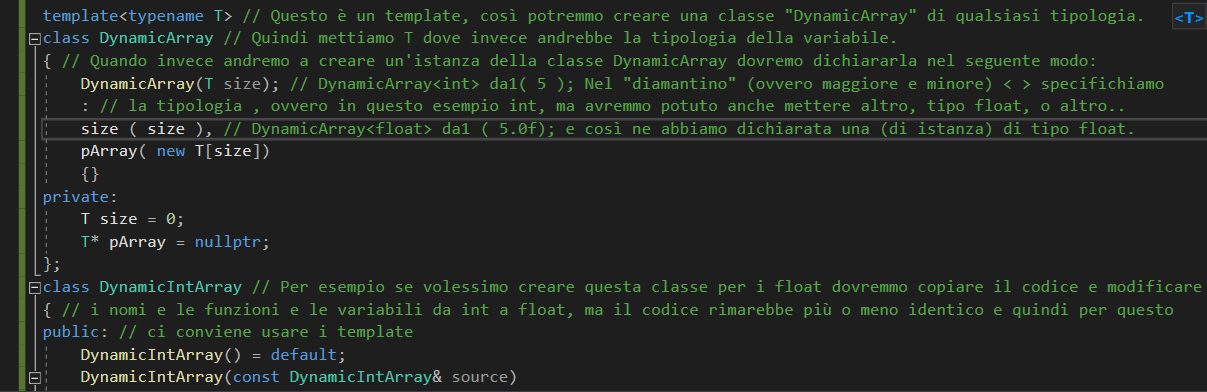
\includegraphics[width=1.2\textwidth, height=1.2\textheight, keepaspectratio]{./imgs/template.png}
	\caption{Template}
	\label{fig:template}
\end{figure}

%TODO: typename

% -------------------------- SECTION: VECTOR -----------------------------------------

%TODO: emplace_back

\section{std::vector<>}

\textsf{\small \textbf{Definizione:} I \textbf{vectors} sono un contenitore rappresentante una array che può cambiare in size (spazio). Sono degli array dinamici.} \\

\textsf{\small I vectors memorizzano i dati in locazioni contigue di memoria e permettono l'accesso diretto a qualsiasi elemento usando l'operatore []. Supportano la riduzione e l'ampiamento dello spazio a runtime (ovvero eseguite mentre il tuo programma è in esecuzione).} \\

\textsf{\small La classe vector fa uso dei template così che possiamo eseguirla con qualsiasi tipo. Per poterla usare avremo bisogno di importare \textbf{\#include <vector>}.} \\

\begin{lstlisting}
	#include <iostream>
	#include <vector>
	
	std::vector<int> v{ 1, 3, 7, 8};
	std::vector<int> v2 = v; // Oppure potevamo scrivere std::vector<int> v2(v);
	
	v2.push_back(9); // Aggiungiamo un elemento.
	
	std::cout << "v size: " << v.size() << std::endl; //Output: v size: 4
	std::cout << "v2 size: " << v2.size() << std::endl; //Output: v2 size: 5
\end{lstlisting}

\textsf{\small Inoltre, la classe vector mette a disposizione tante altre funzioni per la loro manipolazione.} \\

\textsf{\small P.S.: Da non confondere con i vettori in matematica|fisica.} \break

% -------------------------- SECTION: ITERATORI --------------------------------------

\newpage

\section{Iteratori}

\textsf{\small \textbf{Definizione: } Gli \textbf{iteratori} sono degli oggetti (come puntatori) che puntano ad un elemento all'interno di un contenitore. Usiamo gli \textbf{iteratori} per muoverci nel contenitore } \break

\textsf{\small Ci sono diversi tipi di iteratori: } \\

\begin{itemize}
	\item \textsf{\small \textbf{Input Iterators} : Sono i più deboli fra tutti per via delle loro limitate funzionalità. Può essere usato solo in algoritmi single-pass ovvero quelli che processano il contenitore in modo sequenziale.}
	\item \textsf{\small \textbf{Output Iterators} : Anch'essi sono molto limitati. Possono essere usati negli algoritmi single-pass, ma non per accedere agli elementi, ma per essere assegnati agli elementi.}
	\item \textsf{\small \textbf{Forward Iterator} : Sono più in alto nella gerarchia rispetto agli input ed output e possiedono tutte le funzionalità di questi ultimi due, ma possono anche muoversi in avanti ed anch'essi di una posizione alla volta.}
	\item \textsf{\small \textbf{Bidirectional Iterators} : Possiedono tutte le funzionalità degli forward iterators, ma possono muoversi in entrambe le direzioni.}
	\item \textsf{\small \textbf{Random-Access Iterators} : Sono gli iteratori più potenti. Non sono limitati dal solo poter muoversi in modo sequenziale, ma possono accedere in maniera casuale a qualsiasi elemento dentro ad un contenitore. Sono quelli che hanno le stesse funzionalità dei puntatori.}
\end{itemize}

\pagebreak

\begin{figure}[H]
	\centering
	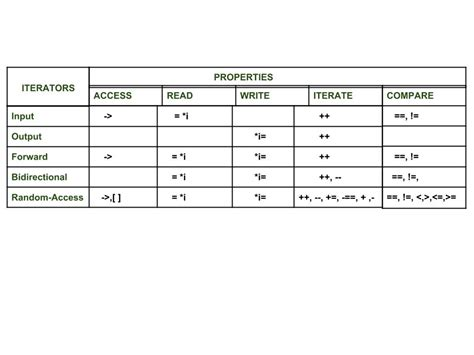
\includegraphics[width=1.2\textwidth, height=1.2\textheight, keepaspectratio]{./imgs/iterators.jpg}
	%\caption{Iteratori}
	\label{fig:iterators}
\end{figure}

\vspace{-3.69cm}

\textsf{\small È sempre meglio usare gli \textbf{iteratori} per iterare tra i contenuti di un contenitore così da evitare di usare l'operatore \textbf{[]} per accedere agli elementi. Inoltre per ottenere la fine di un contenitore con gli \textbf{iteratori} possiamo semplicemente usare la funzione \textbf{end()} al posto di utilizzare lo spazio occupato. } \break

\textsf{\small Possono essere utili per la riusabilità del codice, visto che anche se cambiamo vettore, il codice riguardante gli \textbf{iteratori} non dovrebbe cambiare.} \\

\textsf{\small Gli \textbf{iteratori} ci permettono una manipolazione dinamica dei contenitori, permettendoci di aggiungere e rimuovere elementi in modo dinamico a nostro piacimento.} \break

\textsf{\small Per poter usare gli iteratori è necessario includere \textbf{\#include <iterator>}.} \\

\begin{itemize}
	\item \textsf{\small \textbf{begin()} : Restituisce la posizione iniziale del contenitore.}
	\item \textsf{\small \textbf{end()} : Restituisce la posizione finale del contenitore.}
	%\item \textsf{\small \textbf{} :}
\end{itemize}

\begin{lstlisting}
	#include <iostream>
	#include <iterator>
	
	std::vector<int> v = { 9, 6, 3};
	
	// Dichiaro un iteratore.
	std::vector<int>::iterator it;
	for(it = v.begin(); it < v.end(); it++)
	{
		std::cout << "Elemento: " << *it << std::endl;
	}

	// Output: stampa uno ad uno gli elementi del vettore.
\end{lstlisting}

\begin{itemize}
	\item \textsf{\small \textbf{advance()} : Incrementa la posizione dell'iteratore fino all'argomento passato come parametro.}
	\item \textsf{\small \textbf{next()} : Restituisce un nuovo iteratore dopo aver avanzato di tot posizioni menzionate nell'argomento.}
	\item \textsf{\small \textbf{prev()} : Restituisce un nuovo iteratore dopo essere retrocesso di tot posizioni menzionate nell'argomento.}
	\item \textsf{\small \textbf{inserter()} : Per inserire elementi ad qualsiasi posizione nel contenitore. Prende due argomenti: il contenitore e l'iteratore alla posizione in cui l'elemento deve essere inserito.}
\end{itemize}

\begin{lstlisting}
	#include <iostream>
	#include <iterator>
	
	std::vector<int> v = { 9, 6, 3};
	std::vector<int> v2(2, 5, 8);
	
	std::vector<int>::iterator it = v.begin();
	
	std::advance(it, 2);
	
	std::cout << "Elemento dell'iteratore dopo advance: " << *it << std::endl; // Output: Elemento dell'iteratore dopo advance: 3
	
	std::prev(it, 2);
	std::cout << "Elemento dell'iteratore dopo prec: " << *it << std::endl; // Output: Elemento dell'iteratore dopo prec: 9
	
	std::next(it, 1);
	std::cout << "Elemento dell'iteratore dopo next: " << *it << std::endl; // Output: Elemento dell'iteratore dopo next: 6
	
	// Copio gli elementi di 1 vettore nell'altro usando inserter
	// Inserisco gli elementi di v2 in v alla posizione a cui puntava l'iteratore it.
	std::copy(v2.begin(), v2.end(), std::inserter(v, it));
	
	for(int &x : v)
	{
		std::cout << "Elemento: " << x << std::endl;
	}

	// Output: Gli elementi del vettore con gli elementi aggiunti.
\end{lstlisting}

%TODO: Iterable Interface?

% -------------------------- SECTION: VIRTUAL ----------------------------------------

\newpage

\section{Virtual}

\subsection{Virtual functions}

\textsf{\small \textbf{Definizione:} Una funzione \textbf{virtuale} è una funzione dichiarata in una classe base che può essere ri-definita (\emph{overridden}) da una classe derivata. Le funzioni \textbf{virtuali} ci assicurano che la corretta versione della funzione venga eseguita.} \\

\textsf{\small Alcune regole per le \textbf{funzioni virtuali}: }

\begin{itemize}
	\item \textsf{\small Non possono essere statiche.}
	\item \textsf{\small Può essere una \textbf{friend function} di un'altra classe.}
	\item \textsf{\small Bisognerebbe accedergli attraverso un puntatore o referenza di un tipo alla classe base per ottenere \emph{runtime polymorphism}.}
	\item \textsf{\small Il prototipo della funzione dovrebbe essere lo stesso sia nella classe base sia nella classe derivata.}
	\item \textsf{\small Sono sempre definiti nella classe base e ridefiniti nella classe derivata. Non è obbligatorio che la classe derivata ri-definisca la funzione, può anche soltanto utilizzare quella della classe base.}
	\item \textsf{\small Una classe può avere un \textbf{virtual destructor}, ma non un \textbf{virtual constructor}.}
\end{itemize}

\begin{lstlisting}
	#include <iostream>
	
	class Base {
		public:
			virtual void print()
			{
				std::cout << "print in base class" << std::endl;
			}
		
			void show()
			{
				std::cout << "show in base class" << std::endl;
			}
	};

	class Derived : public Base {
		public:
			void print() override // override non servirebbe, ma aiuta per la manutenzione del codice ed indica che la funzione è stata "overridata".
			{
				std::cout << "print in derived class" << std::endl;
			}
		
			void show()
			{
				std::cout << "show in derived class" << std::endl;
			}
	};

	int main()
	{
		Base* bPtr;
		Derived d;
		bPtr = &d;
		
		// Chiamo la funzione virtuale.
		bPtr->print(); // Output: print in derived class
		
		// Chiamo la funzione non virtuale.
		bPtr->show(); // Output: show in base class
		
		return 0;
	}
\end{lstlisting}

\subsection{Virtual Destructors}

\textsf{\small \textbf{Definizione:} Per rimuovere una classe derivata, la classe base dovrebbe essere definita con un \textbf{distruttore virtuale}. Cancellare una classe derivata usando un puntatore alla classe base senza un distruttore virtuale risulta in un comportamento indefinito (\emph{undefined behaviour}).} \\

\begin{lstlisting}
	#include <iostream>
	
	class A {
		public:
			A()
			{
				std::cout << "Constructor in base class" << std::endl;
			}	
		
			virtual ~A()
			{
				std::cout << "Destructor in base class" << std::endl;
			}
	};

	class B : public A {
		public:
			B()
			{
				std::cout << "Constructor in derived class" << std::endl;
			}
		
			~B()
			{
				std::cout << "Destructor in derived class" << std::endl;
			}
	};

	int main()
	{
		B* bPtr = new B();
		A* aPtr = bPtr;
		
		delete aPtr;
		
		// Output: 
		// Constructor in base class
		// Constructor in derived class
		// Destructor in derived class
		// Destructor in base class
		return 0;
	}
\end{lstlisting}

\textsf{\small In linea di massima, se si ha una funzione virtuale, allora è da mettere anche il distruttore virtuale.} \break

\subsection{Virtual Inheritance}

\textsf{\small \textbf{Definizione:} La \textbf{Ereditarietà virtuale} è usata per risolvere il problema del \textbf{DDD} (\emph{Dreadful Diamond on Derivation}), ovvero quando una classe deriva molteplici classi che derivano dalla stessa classe.} \\

\begin{figure}[H]
	\centering
	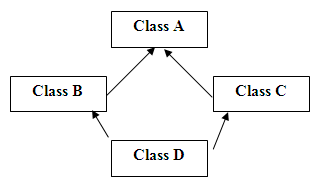
\includegraphics[width=1\textwidth, height=1\textheight, keepaspectratio]{./imgs/diamond_problem2.png}
	\caption{Problema del diamante}
	\label{fig:diamond_problem}
\end{figure}

\textsf{\small Come possiamo notare i dati e le funzioni della \textbf{classe A} è ereditata due volte dalla \textbf{classe D}, una volta per via della \textbf{classe B} e una volta per via della \textbf{classe C}.} \\

\textsf{\small Quando qualsiasi dato o funzione della \textbf{classe A} viene acceduto dalla \textbf{classe D}, nasce dell'ambiguità su quale dato/funzione chiamare. Quella ereditata da \textbf{B} o da \textbf{C}? Questo confonde i compilatori e mostrano errori.}

\textsf{\small Per risolvere questa ambiguità quando la \textbf{classe A} è ereditata sia dalla \textbf{classe B} sia dalla \textbf{classe C}, è dichiarata come \textbf{classe base virtuale} (Fare riferimento all'immagine: \textbf{\ref{fig:diamond_problem}} a \textbf{pag.\pageref{fig:diamond_problem}}).}

\begin{lstlisting}
	#include <iostream>
	
	class A {
		public:
			void show()
			{
				std::cout << "Show from A" << std::endl;
			}
	};

	class B : public virtual A {
	};

	class C : public virtual A {
	};

	class D : public B, public C {
	};

	int main()
	{
		D d;
		d.show(); // Output: Show from A
	}
\end{lstlisting}

\textsf{\small La keyword \textbf{virtual} può essere posta sia prima che dopo \textbf{public}.} \\

%TODO: Pure Virtual

% -------------------------- SECTION: POLYMORPHISM -----------------------------------

\section{Polimorfismo}

\textsf{\small \textbf{Definizione:} La parola \textbf{polimorfismo} significa \emph{avere molte forme}, questo occorre quando c'è una gerarchia di classi e queste sono correlate attraverso l'ereditarietà.} \\

\textsf{\small Ci sono due tipi principali di polimorfismo: }

\begin{itemize}
	\item \textsf{\small \textbf{Compile time Polymorphism} : si ottiene dall'\emph{overloading} di funzioni o di operatori.}
	\item \textsf{\small \textbf{Runtime Polymorphism} : si ottiene dall' \emph{overriding} delle funzioni (con la keyword \textbf{virtual}).}
\end{itemize}

\begin{figure}[H]
	\centering
	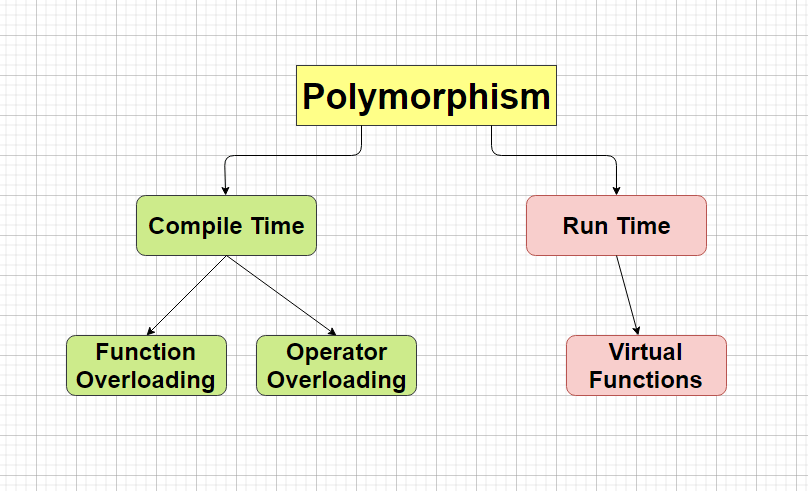
\includegraphics[width=1\textwidth, height=1\textheight, keepaspectratio]{./imgs/polymorphism.png}
	\caption{Polimorfismo}
	\label{fig:polymorphism}
\end{figure}

% -------------------------- SECTION: OVERLOADING --------------------------

\section{Overloading}

\textsf{\small \textbf{Definizione:} L'\textbf{overloading} permette di ridefinire una funzione o un operatore con lo stesso nome e nello stesso scope, ma con una differente implementazione.} \\

\subsection{Function Overloading}

\textsf{\small Si può definire una funzione con lo stesso nome di un'altra purchè abbia argomenti diversi.} \\

\begin{lstlisting}
	void func(int x)
	{
		std::cout << "Valore di x: " << x << std::endl;
	}

	void func(double x)
	{
		std::cout << "Valore di x: " << x << std::endl;
	}

	void func(float x)
	{
		std::cout << "Valore di x: " << x << std::endl;
	}
\end{lstlisting}

\subsection{Operator Overloading}

\textsf{\small Possiamo ridefinire degli operatori per eseguire delle operazioni nel modo che vogliamo noi.} \\

\textsf{\small Utilizziamo la keyword \textbf{operator} ed il simbolo dell'operatore per \emph{overloaddarlo}.} \\

\begin{lstlisting}
	class Vec {
		public:
			Vec(){}
		
			Vec(int x, int y)
			{
				this->x = x;
				this->y = y;
			}
		
			Vector operator+(const Vec& v)
			{
				Vec vec;
				vec.x = this->x + v.x;
				vec.y = this->y + v.y;
				return vec;
			}
		
			int getX()
			{
				return this->x;
			}
		
			int getY()
			{
				return this->y;
			}
		
		private:
			int x;
			int y;
	};

	int main()
	{
		Vec v1(3, 2);
		Vec v2(1, 0);
		
		Vec v3 = v1 + v2;
		
		std::cout << "v3.x: " << v3.getX() << "; v3.getY(): " << v3.y << std::endl;
		// Output: v3.x: 4; v3.y: 2
		// perché facciamo la x di v1 che è 3 + la x di v2 che è 1 quindi 4 e 
		// la y di v1, ovvero 2 + la y di v2, ovvero 0 quindi 2
		// quindi v3 ha membri (4,2).
		return 0;
	}
\end{lstlisting}

\textsf{\small Non tutti gli operatori si possono \emph{overloaddare}.} \\

\textsf{\small Gli operatori che non si possono \emph{overloaddare} sono: \textbf{.} (punto), \textbf{::}, \textbf{?:}(operatore ternario), \textbf{sizeof}.} \\

\subsection{Overloading vs Overriding}

\textsf{\small L'\textbf{overloading} è la creazione di molteplici definizioni di una funzione cambiando la \textbf{signature}: il numero di parametri, la tipologia dei parametri. Il tipo di ritorno non gioca alcun ruolo.} \\

\textsf{\small Può essere fatta sia nelle classi basi che in quelle derivate.} \break

\textsf{\small L'\textbf{overriding} è la ridefinizione di una funzione di una classe base in una classe derivata con la stessa \textbf{signature}, stesso tipo di ritorno e parametri.} \\

\textsf{\small Può essere fatta solo nelle classi derivate.} \break

\textsf{\small Differenza tra \textbf{function overloading} e \textbf{function overriding}: } \break

\begin{tabular}{|c|c|} %TODO: questo è da riguardare, perché la fonte forse ha fatto degli errori.
	\hline
	\textbf{Overloading} & \textbf{Overriding} \\
	\hline
	\textsf{\small Nessuna keyword è usata.} & \textsf{\small Keyword \textbf{override}.} \\
	\hline
	\textsf{\small Il prototipo cambia } & \textsf{\small Il prototipo non cambia.} \\
	\textsf{\small in base ai parametri.} & \textsf{\small } \\
	\hline
	\textsf{\small Occorre durante compile time.} & \textsf{\small Occorre durante runtime.} \\
	\hline
	\textsf{\small I costruttori possono } & \textsf{\small } \\
	\textsf{\small essere "overloaddati".} & \textsf{\small } \\
	\hline
	\textsf{\small I distruttori non } & \textsf{\small I distruttori } \\
	\textsf{\small possono essere "overloaddati".} & \textsf{\small possono essere "overridati".} \\
	\hline
	\textsf{\small } & \textsf{\small Le funzioni virtuali } \\
	\textsf{\small } & \textsf{\small non possono essere "overridate".} \\
	\hline
	\textsf{\small Può essere usato per ottenere } & \textsf{\small Overriding è anche conosciuto come } \\
	\textsf{\small \emph{early binding}.} & \textsf{\small \emph{late binding}.} \\
	\hline
	\textsf{\small La funzione chiamata viene } & \textsf{\small La funzione overriden} \\
	\textsf{\small determinata dal numero} & \textsf{\small è preceduta} \\
	\textsf{\small di parametri.} & \textsf{\small dalla keyword virtual nella classe base.} \\
	\hline
	\textsf{\small Le funzioni verrebbero} & \textsf{\small } \\
	\textsf{\small ridefinite} & \textsf{\small } \\
	\textsf{\small con lo stesso nome, ma} & \textsf{\small } \\
	\textsf{\small differente numero o tipo} & \textsf{\small } \\
	\textsf{\small di parametri.} & \textsf{\small } \\
	\hline
	\textsf{\small } & \textsf{\small L'indirizzo dell'oggetto} \\
	\textsf{\small } & \textsf{\small della classe è assegnato al} \\
	\textsf{\small } & \textsf{\small puntatore la cui funzione} \\
	\textsf{\small } & \textsf{\small è chiamata dal puntatore.} \\
	\hline
	\textsf{\small } & \textsf{\small Quando la funzione è definita viene preceduta} \\
	\textsf{\small } & \textsf{\small dalla keyword virtual nel main.} \\
	%\textsf{\small } & \textsf{\small La stessa funzione è ridefinita } \\
	%\textsf{\small } & \textsf{\small nella classe derivata usando} \\
	%\textsf{\small } & \textsf{\small la keyword \textbf{out}.} \\
	%\textsf{\small } & \textsf{\small } \\
	\hline
\end{tabular}

% -------------------------- SECTION: TIPI DI CAST -----------------------------------

%TODO: Prima di spiegare questi dovrei spiegare i templates, altrimenti uno non capisce i <>.
%TODO: Inoltre dovrei parlare anche della keyword virtual e virtual inheritance.

\newpage

\section{Tipi di Casts}

\textsf{\small \textbf{Definizione:} Il \textbf{casting} è un'operazione che permette la conversione di un valore in un altro. In C++ ci sono diversi tipi di casting: } \\

\subsection{static\_cast<>}

\begin{itemize}
	\item \textsf{\small \textbf{static\_cast<> :} Quello che fa è un cast implicito tra tipi (come int a float, o puntatore a void*) e può anche chiamare funzioni esplicite per la conversione. }
\end{itemize}

\begin{lstlisting}
	float f = 3.69;
	int x = static_cast<int>(f);
	std::cout << "x: " << x << std::endl; // Output: x: 3 
\end{lstlisting}

\subsection{const\_cast<>}

\begin{itemize}
	\item \textsf{\small \textbf{const\_cast<> :} Serve per aggiungere o rimuovere il \textbf{const} ad una variabile. Se la variabile che stiamo cercando di modificare era già const allora questo produce un valore indefinito. Se lo si usa per qualcosa che non era dichiarato come const allora è safe (sicuro farlo, non ci saranno problemi).  }
\end{itemize}

\begin{lstlisting}
	#include <iostream>
	
	void print( char* str)
	{
		std::cout << str << '\n';
	}

	int main()
	{
		const char* c = "testo";
		// Ci serve per poter passare un puntatore a char const ad una funzione che prende un puntatore a char senza const.
		print(const_cast<char*>(c)); // Output: testo
		return 0;
	}
\end{lstlisting}

\subsection{dynamic\_cast<>}

\begin{itemize}
	\item \textsf{\small \textbf{dynamic\_cast<> :} Serve esclusivamente per i casts riguardanti il polimorfismo. Puoi castare un puntatore o una reference a qualsiasi altro tipo di classe. Non solo si può fare un casting verso il basso, ma anche in alto e a lato. Il dynamic\_cast cercherà di ritorna l'oggetto desiderato se possibile, altrimenti ritornerà \textbf{nullptr} in caso di un puntatore e \textbf{std::bad\_cast} nel caso di una reference.}
	\item \textsf{\small Ha delle limitazioni. Non funzionerà nel caso in cui diversi oggetti ereditano tutti dallo stessa classe. (il famoso problema del \emph{dreaded diamond}.) e non stai usando l'ereditarietà \textbf{virtual}.}
	\item \textsf{\small Inoltre può soltanto funzionare con l'ereditarietà pubblica, fallirà con l'ereditarietà \textbf{protected} o \textbf{private}. Comunque questi tipi di ereditarietà sono rare.}
\end{itemize}

\begin{lstlisting}
	// C++ programma per dimostrare che se non c'è
	// alcuna funzione virtuale nella Base classe.
	#include <iostream>
	
	// Base class declaration
	class Base {
		void print()
		{
			std::cout << "Base" << std::endl;
		}
	};
	
	// Derived Class 1 declaration
	class Derived1 : public Base {
		void print()
		{
			std::cout << "Derived1" << std::endl;
		}
	};
	
	// Derived class 2 declaration
	class Derived2 : public Base {
		void print()
		{
			std::cout << "Derived2" << std::endl;
		}
	};
	
	// Driver Code
	int main()
	{
		Derived1 d1;
		
		// Base class pointer hold Derived1
		// class object
		Base* bp = dynamic_cast<Base*>(&d1);
		
		// Dynamic casting
		Derived2* dp2 = dynamic_cast<Derived2*>(bp);
		if (dp2 == nullptr)
			std::cout << "null" << std::endl;
			
		// Output: null, in realtà errore.
		return 0;
	}
\end{lstlisting}

\subsection{reinterpret\_cast<>}

\begin{itemize}
	\item \textsf{\small \textbf{reinterpret\_cast<> :} È quello più pericoloso di tutti e quindi bisogna utilizzarlo con moderazione. Trasforma un tipo direttamente in un altro come cast da un puntatore ad un altro o memorizzare un puntatore in un int, ecc..}
	\item \textsf{\small L'unica cosa garantita con questo tipo di cast è che se torni indietro al tipo originale riotterrai lo stesso valore (non succederà se il tipo era più piccolo del tipo originale.)}
\end{itemize}

\begin{lstlisting}
	class A {
		public:
			int x;
	};

	class B {
		public:
			int x;
	};

	A *a = new A;
	B *b = reinterpret_cast<*B>(a);
	
	a->x = 5;
	std::cout << "b: " << b->x << std::endl; // Output: b: 5
	std::cout << "a: " << a->x << std::endl; // Output: a: 5
\end{lstlisting}

\subsection{C-style \& function-style cast o Regular Cast}

\begin{itemize}
	\item \textsf{\small Questo tipo di cast chiamato \textbf{Regular Cast} o \textbf{C-style cast} (derivando dal C ovviamente) è molto più potente degli altri tipi di cast, ma allo stesso tempo molto meno sicuro.}
	\item \textsf{\small Ignorano i controlli d'accesso quando si esegue uno static\_cast.}
	\item \textsf{\small Permette di fare un cast sicuro ad una classe privata, mentre il suo "equivalente" static\_cast darebbe un errore a tempo di compilazione (compile-time).}
\end{itemize}

\begin{lstlisting}
	double d = 9.87;
	int x;
	
	x = (int)d;
	std::cout << "x: " << x std::endl; // Output: x: 9
\end{lstlisting}

\subsection{Ricapitolando}

\begin{tabular}{|c|c|}
	\hline
	\textbf{Cast} & \textbf{Definizione} \\
	\hline
	\textbf{dynamic\_cast} & \textsf{\small per convertire puntatori/references in una gerarchia di ereditarietà.} \\
	\hline
	\textbf{static\_cast} & \textsf{\small per le conversioni di tipi ordinari.} \\
	\hline
	\textbf{reinterpret\_cast} & \textsf{\small per reinterpretare bit patterns di basso livello. Usare con cauzione.} \\
	\hline
	\textbf{const\_cast} & \textsf{\small per aggiungere/rimuovere \textbf{const} al cast.} \\
	\hline
\end{tabular}

\begin{figure}[ht]
	\centering
	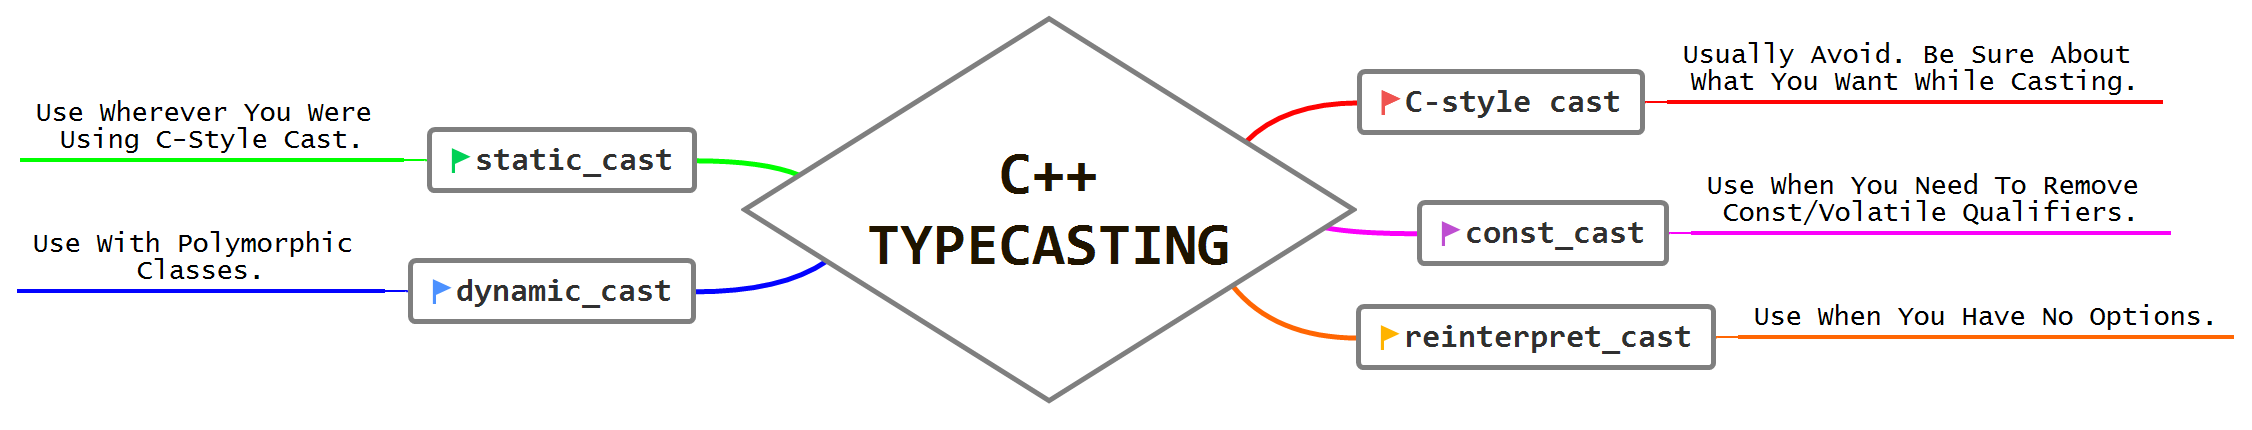
\includegraphics[width=1.2\textwidth, height=1.2\textheight, keepaspectratio]{./imgs/typecasting.png}
	\caption{Typecasting}
	\label{fig:typecasting}
\end{figure}

%TODO: typeid

% -------------------------- SECTION: LAMBDAS ----------------------------------------

%TODO: potrei mettere le lambbdas subito dopo gli iteratori.

\section{Lambdas}

\textsf{\small \textbf{Definizione:} Dal C++11 sono presenti le \textbf{lambdas} che permettono di creare \textbf{funzioni anonime}.} \\

\textsf{\small Servono per creare delle funzioni, dei piccoli frammenti di codice che non hanno bisogno di un nome e non verranno riutilizzati. } \\ % funzioni inline

\textsf{\small Sono una parte centrale della \textbf{programmazione funzionale}.} \\

\textsf{\small Questa è la struttura di una tipica espressione \textbf{lambda} :} \\

\begin{lstlisting}
	[ clausola di cattura ] ( lista di parametri che è opzionale) -> tipoDiRitorno
	{
		// Definizione della lambda.
	}
\end{lstlisting}

\textsf{\small Se nella clausola della cattura è presente un \textbf{=} (uguale), vuol dire che la lambda può accedere a qualsiasi variabile, se c'è un \textbf{\&} vuol dire che stiamo accedendo alle variabili per reference, se la clausola [] è vuota allora può accedere soltanto alle variabili locali, altrimenti lì saranno presenti i nomi delle variabili che si vogliono utilizzare ("catturate" o per valore o per reference).} \\ %TODO: forse si potrebbe rimuovere questa parte e lasciare solo la tabella.

\begin{tabular}{|c|c|}
	\hline
	\textbf{Cattura} & \textbf{Definizione} \\
	\hline
	\textsf{\small []} & \textsf{\small accedere solo alla variabili locali} \\
	\hline
	\textsf{\small [=]} & \textsf{\small accedere a tutte le variabili per valore.} \\
	\hline
	\textsf{\small [\&]} & \textsf{\small accedere a tutte le variabili per reference.} \\
	\hline
	\textsf{\small [nomeVariabile1, \&nomeVariabile2]} & \textsf{\small "cattura" nomeVariabile per valore } \\
	\textsf{\small } & \textsf{\small e nomeVariabile2 per referenza.} \\
	\hline
\end{tabular} \\

\begin{lstlisting}
	#include <iostream>
	#include <vector>
	
	std::vector<int> v1 = { 5, 8, 9, 1, 7};
	std::vector<int> v2 = {12, 36, 27, 92};
	
	// Lambda.
	auto pushinto = [&](int m)
	{
		v1.push_back(m);
		v2.push_back(m);
	}; // Da notare il ; alla fine.

	// Pusha in entrambi v1 e v2 il numero 24
	pushinto(24);
	
	// Lambda, accediamo a v1 per valore (quindi ne facciamo una copia).
	[v1]()
	{
		for(auto p = v1.begin(); p != v1.end(); p++)
		{
			std::cout << *p << std::endl;
		}
	};

	int n = 7;
	// trova il primo numero maggiore di n.
	// [n] significa che stiamo accedendo e possiamo soltanto accedere ad n (per valore, ovvero una copia di essa).
	std::vector<int>:: iterator p = std::find_if(v1.begin(), v1.end(), [n](int i)
	{
		return i > n;
	});

	std::cout << "Il primo numero maggiore di n e\': " << *p << std::endl; // Output: Il primo numero maggiore di n e\': 8

	// Qui [=] vuol dire che possiamo accedere a tutte le variabili.
	int countN = std::count_if(v1.begin(), v1.end(), [=](int a) 
	{
		return a >= n;
	});

	std::cout << "Il numero di elementi piu' grandi o uguali ad n sono: " << countN << std::endl; // Output: Il numero di elementi più grandi o uguali ad n sono: 4 (perchè abbiamo inserito anche il 24 nell'operazione precedente).
\end{lstlisting}

%TODO: capture.
%TODO: poi trattare anche dei functors.

% -------------------------- SECTION: MEMORIA DINAMICA -------------------------------

\newpage

\section{Memoria dinamica}

\textsf{\small \textbf{Definizione: } Riguarda l'allocazione di memoria manualmente da parte del programmatore. La memoria allocata dinamicamente è allocata nell' \textbf{Heap} mentre le variabili locali e la memoria non statica viene allocata nello \textbf{Stack}.}

\begin{itemize}
	\item \textsf{\small \textbf{Heap} : memoria dinamica.}
	\item \textsf{\small \textbf{Stack} : variabili locali e non-statiche.}
\end{itemize}

\subsection{Memoria Dinamica in C}

\textsf{\small In C per l'allocazione dinamica della memoria usufruivamo di 4 diverse funzioni: \textbf{malloc()} (per allocare), \textbf{calloc()}, \textbf{realloc()} (per riallocare), \textbf{free()} (per liberare la memoria).} \\

\textsf{\small Tutte questi funzioni del C, esistono anche nel C++, ma questo ha un suo modo per l'allocazione dinamica della memoria.} \break

\subsection{new e delete}

\subsubsection{new}

\textsf{\small \textbf{Definizione: } L'operatore \textbf{new} denota una richiesta di allocazione di memoria nello spazio libero. Se sufficiente memoria è disponibile, l'operatore inizializza la memoria e restituisce l'indirizzo della nuova memoria allocata ed inizializzata al puntatore.} \\

\begin{lstlisting}
	// Esempio 1
	int *ptr = nullptr;
	ptr = new int;
	
	// Esempio 2
	double *dPtr = new double;
	
	// Esempio 3
	int *p = new int(22);
	
	// Esempio 4
	int *pArray = new int[12];
\end{lstlisting}

\subsubsection{array normali vs array con la new}

\textsf{\small L'unica differenza è che gli array normali vengono deallocati dal compilatore, mentre quelli creati con la new devono essere deallocati dal programmatore.} \break

\subsubsection{delete}

\textsf{\small \textbf{Definizione: } Utilizziamo la keyword \textbf{delete} per deallocare la memoria precedentemente allocata.} \\

\begin{lstlisting}
	// Esempio 1
	int *ptr = new int;
	
	delele ptr;
	
	// Esempio 2
	int *p = new int[6];
	
	delete[] p;
\end{lstlisting}

\subsection{Evitare di usare new}

\textsf{\small \textbf{Definizione: } Ci sono vari motivi per cui evitare o minimizzare gli utilizzi della keyword \textbf{new}: } \\

\begin{itemize}
	\item \textsf{\small Il C++ non ha un garbage collector, quindi per ogni \textbf{new} ci deve essere una corrispondente \textbf{delete}.}
	\item \textsf{\small Se viene lanciata un'eccezione poi la memoria non viene mai liberata.}
	\item \textsf{\small Dovrebbe essere tutto nel distruttore, concetto del \emph{RAII}.} %TODO: add ref quando ne parlerò.
	\item \textsf{\small Se restituisci per esempio una stringa a qualcuno, ora sono loro a doverla cancellare (con la \textbf{delete}). E se a loro volta la passassero come argomento? Quando dovrebbe essere liberata? (con \textbf{delete}).}
	\item \textsf{\small Può essere un problema nel multi-threading.}
	\item \textsf{\small Potrebbe portare a dei \emph{memory leaks}.}
\end{itemize}

% -------------------------- SECTION: RAII -------------------------------------------

\section{RAII | Resource Acquisition is initialization}

\textsf{\small \textbf{Definizione: } \textbf{RAII} (\emph{Resource Acquisition is Initialization}) è un idioma comune della programmazione e della gestione delle risorse. Ogni allocazione della risorsa è fatta alla creazione dell'oggetto da parte del \textbf{costruttore} mentre la deallocazione (rilascio della memoria) viene fatto dal \textbf{distruttore}. Quindi se non ci sono leaks all'oggetto, non ci sono leaks nemmeno alla risorse. } \\

\begin{figure}[ht]
	\centering
	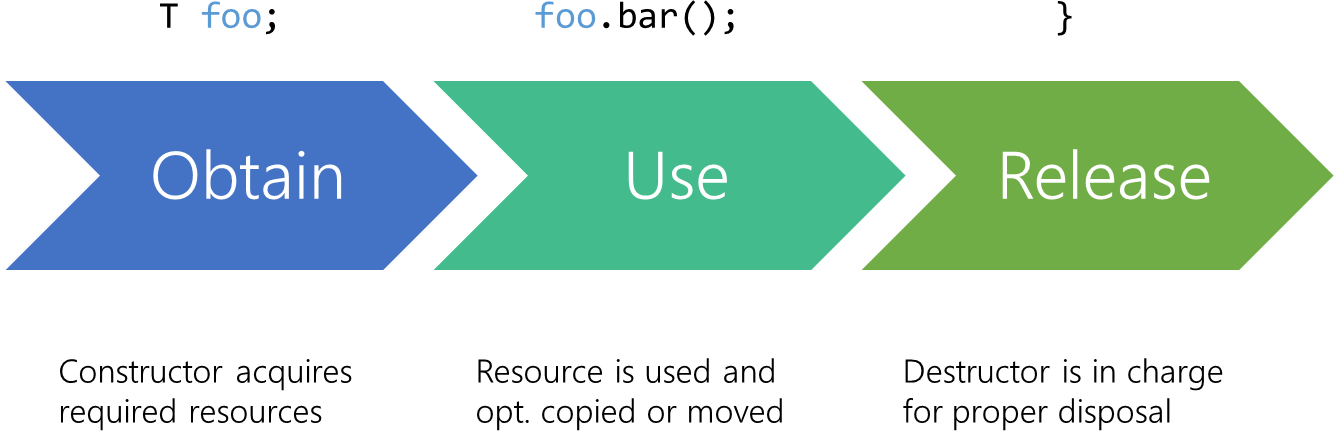
\includegraphics[width=1\textwidth, height=1\textheight, keepaspectratio]{./imgs/RAII.png}
	\caption{RAII}
	\label{fig:RAII}
\end{figure}

%TOOD: magari approfondire l'argomento.

% -------------------------- SECTION: TIPI DI COSTRUTTORI | RULE OF 3 ----------------

\section{Constructor types | Rules of}

\subsection{Rule of Zero}

\textsf{\small \textbf{Definizione: } La \textbf{regola dello zero} (è una regola generale/un'indicazione) afferma che se non hai bisogno di nessuno di questi, allora non ne devi implementare nessuno: } \\

\begin{itemize}
	\item \textsf{\small \textbf{Distruttore} : libera tutte le risorse precedentemente allocate.}
	\item \textsf{\small \textbf{Copy Constructor} : Fa una copia di un oggetto.}
	\item \textsf{\small \textbf{Copy assign} : overload dell'operatore di assegnamento.}
\end{itemize}

\subsection{Copy Constructor}

\textsf{\small \textbf{Definizione: } Il \textbf{Copy Constructor} è un tipo di costruttore che inizializza un oggetto usando un altro oggetto della stessa classe.} \\

\textsf{\small Un costruttore di copia ha la seguente struttura: } \\

\begin{lstlisting}
	// È un costruttore quindi si chiama con il nome della classe.
	NomeDellaClasse(const NomeDellaClasse &vecchioOggetto);
\end{lstlisting}

\textsf{\small Un copy constructor potrebbe essere chiamato per:}

\begin{enumerate}
	\item \textsf{\small Quando un oggetto della classe è ritornato per valore.}
	\item \textsf{\small Quando un oggetto della classe è passato come argomento ad una funzione per valore.}
	\item \textsf{\small Quando un oggetto è costruito sulla base di un altro oggetto.}
	\item \textsf{\small Quando il compilatore genera un oggetto temporaneo.}
	%\item \textsf{\small }
\end{enumerate}

\begin{lstlisting}
	class Point {
		public:
			// Costruttore normale
			Point(int x, int y)
			{
				this->x = x;
				this->y = y;
			}
			
			// Copy Constructor
			// Assiegnamo i valori di x ed y in base ai valori di un'istanza p della classe Point.
			Point(const Point &p)
			{
				this->x = p.x;
				this->y = p.y;
			}
		
			int getX() { return this->x };
			int getY() { return this->y };
		
		private:
			int x;
			int y;
	};

	int main()
	{
		Point p1(3, 5); // Il costruttore normale viene chiamato qui.
		Point p2 = p1; // Il Copy Constructor viene chiamato qui.
		
		std::cout << "p1.x: " << p1.getX() << ", p1.y: " << p1.getY() << "\n"; // Output: p1.x: 3, p1.y: 5
		std::cout << "p2.x: " << p2.getX() << ", p2.y: " << p2.getY() << "\n"; // Output: p2.x: 3, p2.y: 5
		
		return 0;
	}
\end{lstlisting}

\subsection{Copy Assign}

\textsf{\small \textbf{Definizione: } Il \textbf{copy assignment operator} è ciò che ti permette di assegnare, di copiare un'istanza e di portare i suoi dati in un' altra istanza.} \\

\textsf{\small È usato per rimpiazzare i dati di un oggetto precedentemente inizializzato con i dati di qualche altro oggetto.} \\

\textsf{\small Se non si dichiara un \textbf{assignment operator} allora il compilatore provvederà a fornirtene uno automaticamente.} \\

\textsf{\small In linea di massima, se hai bisogno di un \textbf{copy constructor} allora avrai bisogno anche di un \textbf{copy assignment operator}.} \\

%TODO: da riguardarsi il copy assignment operator nel codice.
\begin{lstlisting}
	class Point {
		public:
			// Normal Constructor
			Point(int x, int y)
			{
				this->x = x;
				this->y = y;
			}
		
			// Copy Constructor
			Point(const Point& p)
			{
				this->x = p.x;
				this->y = p.y;
			}
		
			// Copy Assignment
			Point& operator=(const Point& p)
			{
				this->x = p.x;
				this->y = p.y;
				return *this;
			}
			
			int getX() { return this->x };
			int getY() { return this->y };
			
		private:
			int x;
			int y;
	};
\end{lstlisting}

%TODO: copy constructor = delete, copy assignment = delete.

\subsection{=default | Defaulted Functions}

\textsf{\small \textbf{Definizione: } Le \textbf{defaulted functions} in modo esplicito permette di aggiungere \textbf{=default} alla fine di una funzione per dichiararla una \emph{funzione default esplicita}. Questi sono più efficienti.} \\

\begin{lstlisting}
	class A {
		public:
		A(int a)
		{
			this->a = a;
			this->b = 0;
		}
	
		A(int a, int b) = default
		{
			this->a = a;
			this->b = b;
		};
	
		// Non ci sarebbe bisogno di mettere =default al costruttore A(), perché questo è già il costruttore di default.
		A(); 
		
		int a;
	};

	int main()
	{
		// Eseguito usando il default constructor
		A a(2);
		
		// Eseguito usando il costruttore parametrizzato.
		A b(5, 7);
		return 0;
	}
\end{lstlisting}

\subsection{=delete | Deleted Functions}

\textsf{\small \textbf{Definizione: } Apparte, deallocare la memoria, dal C++11 la \textbf{delete} ha un nuovo significato: \emph{disabilitare l'utilizzo di una funzione membra}. Queste funzioni sono conosciute come \textbf{funzioni deleted esplicitamente}.} \\

\begin{lstlisting}
	class A {
		public:
			A(int a): x(a)
			{
				this->a = a;
			}
		
			// Disabilitare il copy constructor.
			A(const A& ) = delete;
			
			// Disabilitare il copy assignment operator.
			A& operator=(const A& ) = delete;
			
			int x;
	};

	int main()
	{
		A a1(3), a2(6), a3(9);
		
		// Errore, l'utilizzo del copy assignment operator è disabilitato.
		a1 = a2;
		
		// Errore, l'utilizzo del copy constructor è disabilitato.
		a3 = A(a2);
		return 0;
	}
\end{lstlisting}

\textsf{\small \textbf{Ma qual è l'utilità di far ciò?}} \\

\begin{enumerate}
	\item \textsf{\small Previene il compilatore dal generare le \textbf{special member functions} (costruttori, distruttori, copy constructor, ecc..) che non vogliamo.} \\
	\item \textsf{\small Il disabilitare le normali funzioni membro o non-membro previene problemi di promozioni di tipo dal causare una chiamata involontaria alla funzione.} \\
	%\item \textsf{\small } \\
\end{enumerate}

\subsection{Copy Constructor vs Copy Assignment Operator}

\begin{tabular}{|c|c|}
	\hline
	\textbf{Copy Constructor} & \textbf{Copy Assignment Operator} \\
	\hline
	\textsf{\small È chiamato quando una } & \textsf{\small È chiamato quando ad un oggetto } \\
	\textsf{\small nuova istanza viene creata da } & \textsf{\small già inizializzato gli viene } \\
	\textsf{\small un oggetto già esistente, } & \textsf{\small assegnato un nuovo valore } \\
	\textsf{\small come copia di questo.} & \textsf{\small da un oggetto già esistente.} \\
	\hline
	\textsf{\small Crea un nuovo blocco di memoria} & \textsf{\small Non crea un nuovo blocco di memoria.} \\
	\textsf{\small per il nuovo oggetto.} & \textsf{\small } \\
	\hline
	\textsf{\small È un costruttore overloaded.} & \textsf{\small È un operatore bitwise.} \\
	\hline
	\textsf{\small Il compilatore fornisce} & \textsf{\small Una copia bitwise viene creata} \\
	\textsf{\small implicitamente un copy constructor} & \textsf{\small se l'assignment operator} \\
	\textsf{\small se uno non ne esiste già.} & \textsf{\small non viene overloaded.} \\
	%\textsf{\small } & \textsf{\small } \\
	\hline
\end{tabular}

\subsection{Rule of Three}

\textsf{\small \textbf{Definizione: } La \textbf{regola dei tre}, essenzialmente, afferma che se uno (o anche più) tra questi è definito, allora tutti e tre dovrebbero essere definiti: } \\

\begin{itemize}
	\item \textsf{\small \textbf{Distruttore} : libera tutte le risorse precedentemente allocate.}
	\item \textsf{\small \textbf{Copy Constructor} : Fa una copia di un oggetto.}
	\item \textsf{\small \textbf{Copy assignment operator} : overload dell'operatore di assegnamento.}
\end{itemize}

\textsf{\small I costruttori e gli assignment operator generati implicitamente fanno una \textbf{shallow copy} (copia dei dati di tutte le variabili dell'oggetto originale. Ha problemi se i dati son allocati con memoria dinamica, in quel caso faranno referenza alla stessa locazione di memoria) dei dati membri. Noi abbiamo bisogno di una \textbf{deep copy} (copia dei dati di tutte le variabili e alloca simili risorse di memoria con lo stesso oggetto) quando la classe contiene puntatori che puntano a risorse di memoria allocate dinamicamente.} \\

\subsection{Move Constructor}

\textsf{\small \textbf{Definizione: } } \\

\subsection{Move Assignment Operator}

\textsf{\small \textbf{Definizione: } } \\

\subsection{Rule of Five}

\textsf{\small \textbf{Definizione: } La \textbf{regola dei cinque} è applicata per la gestione delle risorse. Se uno (o più) fra questi 5 viene implementato e le \textbf{move semantics} sono desiderate allora vanno implementate tutte e 5. } \\

\begin{itemize}
	\item \textsf{\small \textbf{Distruttore} : libera tutte le risorse precedentemente allocate.}
	\item \textsf{\small \textbf{Copy Constructor} : Fa una copia di un oggetto.}
	\item \textsf{\small \textbf{Copy assignment operator} : overload dell'operatore di assegnamento.}
	\item \textsf{\small \textbf{Move Constructor} : Al posto di copiare come il copy constructor, trasferisce le risorse e pone a null i puntatori degli oggetti temporanei.}
	\item \textsf{\small \textbf{Move Assignment Operator} : Si può usare un move assignment operator per trasferire la proprietà da un oggetto ad un altro.}
\end{itemize}

\begin{figure}[ht]
	\centering
	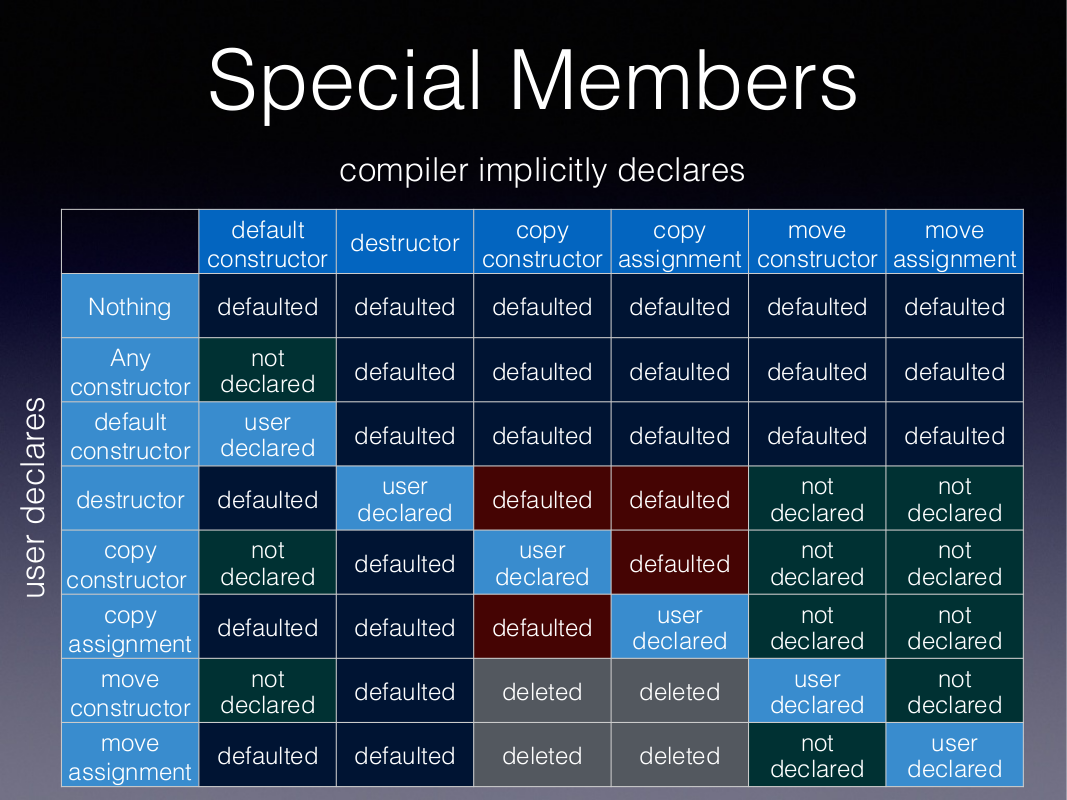
\includegraphics[width=1\textwidth, height=1\textheight, keepaspectratio]{./imgs/rule_of_five.png}
	\caption{Rule of Five}
	\label{fig:rule_of_five}
\end{figure}

%TODO: codice

%TODO: explicit keyword?

% -------------------------- SECTION: MOVE SEMANTICS ---------------------------------

\section{Move Semantics}

\textsf{\small \textbf{Definizione: } } \\

% -------------------------- SECTION: CLASSI ASTRATTE --------------------------------

%TODO: abstract
%TODO: Pure Virtual

\section{Classi Astratte}

\textsf{\small \textbf{Definizione: } } \\

% -------------------------- SECTION: ECCEZIONI --------------------------------------

%TODO: try/catch
%TODO: Errori a compile-time ed errori a runtime.
%TODO: throw.
%TODO: std::throw exception

\section{Eccezioni}

\textsf{\small \textbf{Definizione: } } \\

% -------------------------- SECTION: OPERAZIONI SU FILE -----------------------------

%TODO: numeri pseudo-random?
%TODO: std::chrono

\section{Operazioni su file}

\textsf{\small \textbf{Definizione: } } \\